\setRL
\pagenumbering{arabic} 


\section{\label{sec:nuclearenvelope}
بسته‌ی هسته‌ی سلول
}
غشای هسته یا نام رایج آن، بسته‌ی هسته
\LTRfootnote{nuclear envelope}
ساختاری متفاوت نسبت به غشای سلول دارد. در خارج و اطراف هسته، ساختارهای زیادی وجود دارد، مانند شبکه‌ی اکتین
\LTRfootnote{actin network}
 و میکروتیوبول‌ها
\LTRfootnote{microtubules}
. هسته‌ی سلول از طریق بسته‌ی هسته با تمامی‌ ارگان‌های لازم در ارتباط است. در شکل 
\ref{fig:nuclearenvelope}
نقاشی از ساختار کلی بسته‌ی هسته نشان داده شده. از بالا به پایین، خطوط زرد رنگ نماینده‌ی شبکه‌ی پروتئینی اکتین است. این شبکه از تریق پروتئین‌های روی بسته‌ی هسته به نام نسپرین
\LTRfootnote{nesprin}
به بسته‌ی هسته متصل است و پلی برای انتقال نیرو‌های خارج از سلول به هسته‌ی سلول است
\cite{Lammerding2011}
. بسته‌ی هسته از ۲ عدد غشای لیپیدی دو لایه (نوارهای صورتی) با نام غشای بیرونی و غشای داخلی تشکیل شده است. ضخامت فضای بین دو غشا از ۲۰ تا ۴۰ نانومتر تغییر می‌کند. میان دو غشا مایع شبیه به سیتوپلاسم و همچنین شبکه‌ی پروتئینی برای انتقال مواد بین هسته و سلول وجود دارد. پروتئین‌های نسپرین همچنین در غشای داخلی هم حضور دارند و غشای داخلی را به شبکه‌ی پروتئینی لمینا
\LTRfootnote{lamina}
متصل می‌کنند. لمینا‌ شبکه‌ای است به ضخامت حدود ۵۰ تا ۸۰ نانومتر که تمام سطح غشای داخلی را پوشانده است. در تصویر سمت راست شکل 

با استفاده از روش‌های رنگامیزی میکروسکوپی، لایه‌ی لمینا را به رنگ سبز روشن می‌بینیم که کروماتین‌های (قرمز) درون هسته را محصور کرده‌اند. لمینا خاصیت الاستیکی دارد و تقریبا تمام ویژگی الاستیکی بسته‌ی هسته به علت وجود این بخش است
\cite{Steensel2017wd}
. 


\begin{figure}[h]
\begin{center}
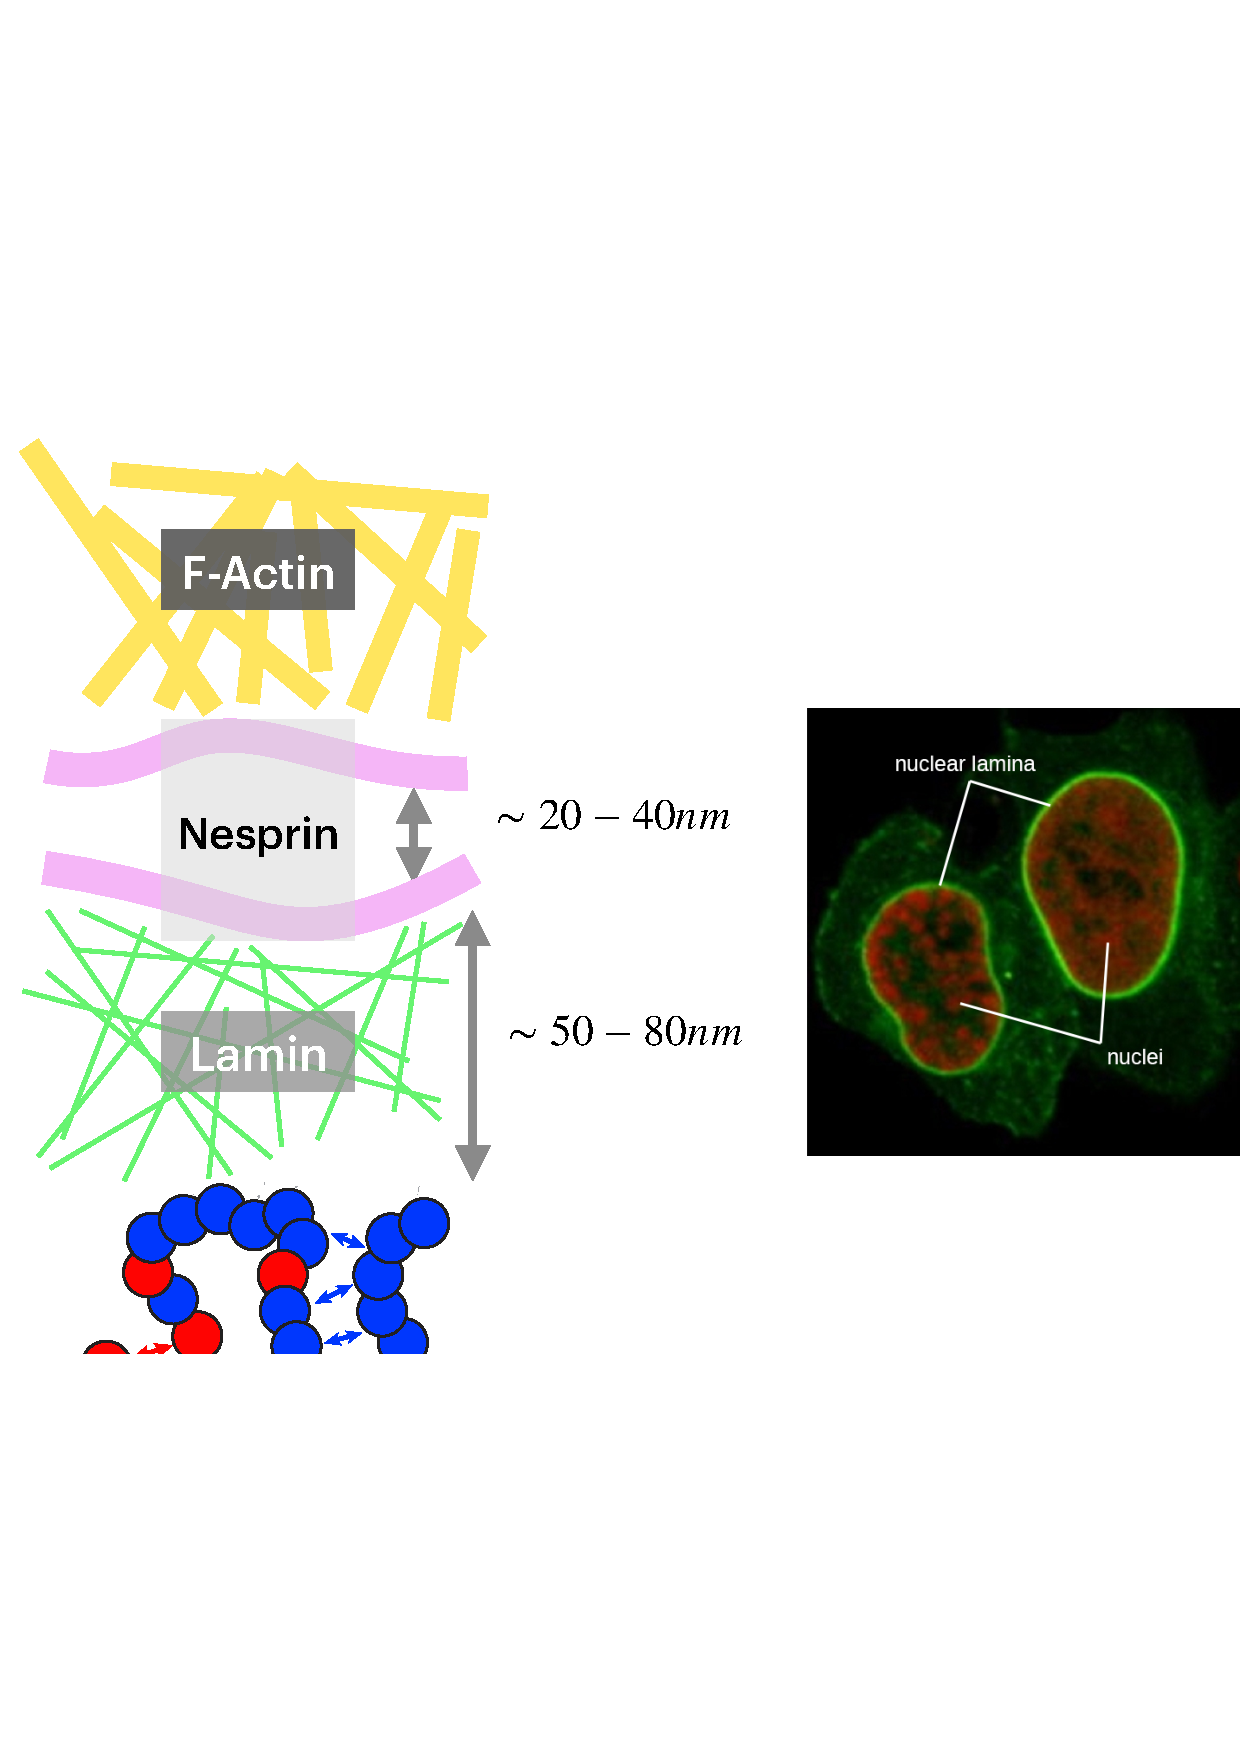
\includegraphics[width=3.5in]{\MemBio /Pics/NuclearEnvelope}
\caption{
عکس سمت راست، تصویر رنگامیزی شده‌ی هسته. لایه‌ی لمینا با رنگ سبز روشن، و کروماتین‌های درون هسته با رنگ قرمز نمایش داده‌ شده‌اند. شکل سمت چپ، نقاشی بسته‌ی هسته از بالا به پایین: شبکه‌ی اکتین که با پروتئین‌های نسپرین به غشای دولایه‌ی بیرونی (نوار صورتی) متصل شده‌اند. غشای داخلی نیز به کمک همین پروتئین به لایه‌ی لمینا متصل شده. فضای میان غشای داخلی و خارجی از ۲۰ تا ۴۰ نانومتر تغییر می‌کند. ضخامت لمینا نیز بین ۵۰ تا ۸۰ نانومتر است. کروماتین‌های درون هسته نیز (دایره‌های آبی و قرمز) با لایه‌ی لمینا اتصالاتی برقرار می‌کنند. 
}
\label{fig:nuclearenvelope}
\end{center}
\end{figure}
مدول الاستیک شبکه‌ی اکتین تقریبا ۵۰۰ پاسکال، و مدول الاستیک هسته‌ی سلول درون سلول، ۵ هزار پاسکال و هنگامی ‌که از سلول خارج شده باشد، ۸ هزار پاسکال اندازه‌گیری شده‌است
\cite{Dahl2004, CAILLE2002177}
.







